\documentclass[11pt,letterpaper]{article}

\usepackage{pgfgantt}
\usepackage[letterpaper,margin=0.75in,nohead]{geometry}
\usepackage{graphicx}
\usepackage{subcaption}
\usepackage[colorlinks]{hyperref}
\usepackage{url}
\usepackage{filecontents}
\usepackage{breakurl}

\hypersetup{
    colorlinks,
    linkcolor={red},
    citecolor={red},
    urlcolor={blue}
}

% add packages as needed



\begin{filecontents*}{hope2.bib}
	@article{Jiechieu2021,
		author={Jiechieu, Kameni Florentin Flambeau
			and Tsopze, Norbert},
		title={Skills prediction based on multi-label resume classification using CNN with model predictions explanation},
		journal={Neural Computing and Applications},
		year={2021},
		month={May},
		day={01},
		volume={33},
		number={10},
		pages={5069-5087},
		issn={1433-3058},
		doi={10.1007/s00521-020-05302-x},
		url={https://doi.org/10.1007/s00521-020-05302-x}
	}

	@misc{zimmermann2016datadriven,
		title={Data-driven HR - Resume Analysis Based on Natural Language Processing and Machine Learning}, 
		author={Tim Zimmermann and Leo Kotschenreuther and Karsten Schmidt},
		year={2016},
		eprint={1606.05611},
		archivePrefix={arXiv},
		primaryClass={cs.CL}
	}
	
	@article{Rasheed2021,
		author = "Khansa Rasheed and Adnan Qayyum and Mohammed Ghaly and Ala Al-Fuqaha and Adeel Razi and Junaid Qadir",
		title = "{Explainable, Trustworthy, and Ethical Machine Learning for Healthcare: A Survey}",
		year = "2021",
		month = "4",
		url = "https://www.techrxiv.org/articles/preprint/Explainable_Trustworthy_and_Ethical_Machine_Learning_for_Healthcare_A_Survey/14376179",
		doi = "10.36227/techrxiv.14376179.v1"
	}
	
	@misc{sinha2021perturbing,
		title={Perturbing Inputs for Fragile Interpretations in Deep Natural Language Processing}, 
		author={Sanchit Sinha and Hanjie Chen and Arshdeep Sekhon and Yangfeng Ji and Yanjun Qi},
		year={2021},
		eprint={2108.04990},
		archivePrefix={arXiv},
		primaryClass={cs.CL}
	}
		
	@article{garreau2020explaining,
		title={Explaining the Explainer: A First Theoretical Analysis of LIME}, 
		author={Damien Garreau and Ulrike von Luxburg},
		year={2020},
		eprint={2001.03447},
		archivePrefix={arXiv},
		primaryClass={cs.LG}
	}

	@article{ribeiro2016why,
		title={"Why Should I Trust You?": Explaining the Predictions of Any Classifier}, 
		author={Marco Tulio Ribeiro and Sameer Singh and Carlos Guestrin},
		year={2016},
		eprint={1602.04938},
		archivePrefix={arXiv},
		primaryClass={cs.LG}
	}

	@article{dataset,
		title={"https://github.com/florex/resume_corpus/blob/master/resumes_corpus.zip}, 
	}
	
	
	
\end{filecontents*}

\title{CIS 6930: Trustworthy Machine Learning\\
	\Large Project Proposal: Decrypting job title classification model} %% TODO: replace with the title of your project

%% TODO: your name and email go here (all members of the group)
%% Comment out as needed and designate a point of contact
\author{
        Tanvi Jain \\{\em (Point of Contact)} \\
        tjain@ufl.edu\\
        \and
        Nimish Bajaj \\
        nimishbajaj@ufl.edu\\
}

% set the date to today
\date{\today}


\begin{document} % start document tag

\maketitle


%%% Remember: writing counts! (try to be clear and concise.)
%%% the whole proposal should be about 2 s (in 11pt font)


%% TODO: write your introduction
%% Must address:
%% - What is the problem?
%% - Why is the problem interested and worth solving?
%% - What are you proposing to do (at high level)?
%%
\section{Introduction}

% TODO:

Determine whether explainable/interpretable ML techniques like LIME and others can provide useful insights into the cause of the unfairness.

A model's accuracy is not always enough to state whether it will perform well in the wild because the accuracy highly depends on the data that was used to train and test the model. 
Explaining the results of a model, and identifying what leads to a particular classification can help provide insights into the model.
Once you add interpretability to the model, its result can be easily understood by a domain expert can be verified for correctness. This greatly enhances the trustworthiness of the model.


We are proposing to build a text classification model and explaining the results using LIME, and validate if LIME can provide stable and meaningful features. 


%% TODO: write your background and related work
%% Must contain:
%% - Background to make the proposal self-contained
%% - Short related work survey (what are the 3-4 most related papers about? what do they do?)
%% - Why is your proposal novel? What are you proposing to do different?
%%
\section{Background and Related Work}

Model interpretation techniques have been in place for the last couple of years, but they are not always able to provide stable inferences for a given problem. 
Work done on inference healthcare model\cite{Rasheed2021}, Perturbing Inputs for Fragile Interpretations in Deep Natural Language Processing \cite{sinha2021perturbing} and many more have a common objective, i.e. to have robust interpretations for determining the trustworthiness of the model.

For our project, we are planning to decrypt the Job classification model on \href{https://github.com/florex/resume_corpus/blob/master/resumes_corpus.zip}{Resume corpus}. Our work will include categorizing resumes using CNN and RNN. We are going to train Neural Network and use the inference technique 'LIME'. Since the data contains technical words which are sometimes outside of the English vocabulary, we are going to tune word embedding for the problem domain.


Existing work has explored a CNN for training a classification model, as part of the project we will be using an RNN to learn the temporal features. The data contains technical words which are sometimes outside of the English vocabulary, we are going to tune word embedding for the problem domain by utilizing the training dataset and other datasets from the same domain.


% TODO:


%% TODO: write your proposed approach and describe your plan
%%
%% - Describe your approach to solve the problem
%% - What's your plan?
%% - Be concrete!!
%% 		-- What dataset will you use?
%% 		-- What equipment do you need? How will you get it?
%% 		-- What are you going to measure? What metrics will you use?
%%		-- How will you know whether what you are doing is working?
%% 
\section{Proposed Approach \& Plan}

% TODO:


%% TODO: Write a short timeline of your project
%%
%% - Describe steps and milestones for you project
%% - Briefly state what you hope the final outcome will be. (Will you have preliminary results to include on the presentation/poster?)
%%
%%
%% Keep in mind the project milestones must include mid semester report
%%

Following is the approach we are going to take:


1. Fetch data and take samples as per the distribution of data for train, test, and validation

2. Clean and vectorize the data for Neural Network (NN) approach

3. Build a NN architecture to learn classification labels

4. Train, test, and validate the neural network

5. Use LIME for model inferencing

6. Manually validate LIME output


For the test and experimentation, we are currently foreseeing that the local machine would be sufficient for carrying out the work. If needed we will use the hyper-gator resources that are availed to us as part of this project. 

\begin{figure}[h!]
	\centering
	\begin{subfigure}[b]{0.45\linewidth}
		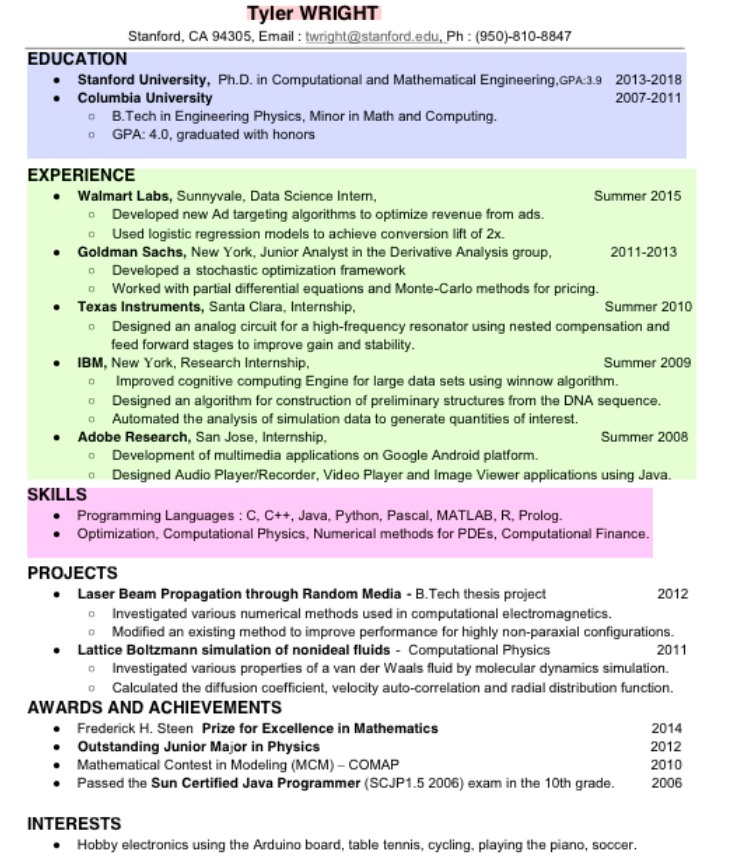
\includegraphics[width=\linewidth]{images/resume.png}
		\caption{Example Input}
	\end{subfigure}
	\begin{subfigure}[b]{0.45\linewidth}
		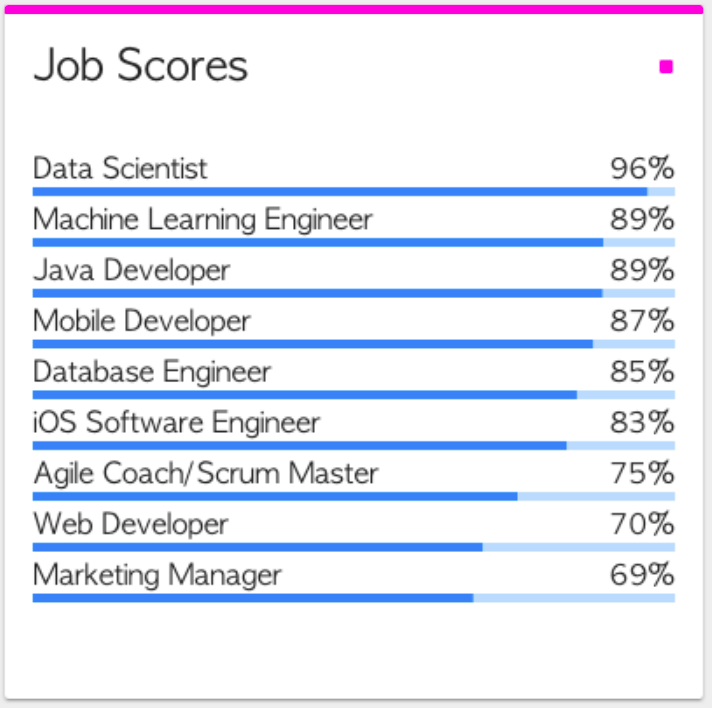
\includegraphics[width=\linewidth]{images/job_title.png}
		\caption{Model prediction}
	\end{subfigure}
	\caption{Model output description \cite{Rasheed2021}}
	\label{fig:coffee}
\end{figure}


\section{Timeline}

% TODO:
\begin{figure}[h!]
	
	
	\begin{center}
		
		\begin{ganttchart}[y unit title=0.4cm,
			y unit chart=0.5cm,
			vgrid,hgrid, 
			title label anchor/.style={below=-1.6ex},
			title left shift=.05,
			title right shift=-.05,
			title height=1,
			progress label text={},
			bar height=0.7,
			group right shift=0,
			group top shift=.6,
			group height=.3]{1}{30}
			%labels
			\gantttitle{September 27 - December 7}{30} \\
			\gantttitle{Week1}{3} 
			\gantttitle{Week2}{3} 
			\gantttitle{Week3}{3} 
			\gantttitle{Week4}{3} 
			\gantttitle{Week5}{3} 
			\gantttitle{Week6}{3} 
			\gantttitle{\color{red}Mid Sem}{3}
			\gantttitle{Week8}{3} 
			\gantttitle{Week9}{3} 
			\gantttitle{Week10}{3} \\
			%tasks
			\ganttbar{Research}{1}{6} \\
			\ganttbar{Data sampling}{4}{7} \\
			\ganttbar{Data preprocessing}{6}{12} \\
			\ganttbar{NN architecture}{10}{15} \\
			\ganttbar[]{Model training}{15}{22} \\
			\ganttbar{Model inferencing}{22}{26} \\
			\ganttbar{LIME validation}{24}{28} \\
			\ganttbar[]{Output generation}{27}{30}
			
		\end{ganttchart}
	\end{center}
	\caption{Project Timeline}
\end{figure}


%%%%
\nocite{*}
\bibliography{hope2}
\bibliographystyle{plain}


\end{document} % end tag of the document
